\section{Contraceptive Method Choice}
\label{db:sec:ds1}
\subsection{Description}
Contraceptive Method Choice contains the results of a survey. The samples are married women who were either not pregnant or do not know if they were at the time of interview. The problem is to predict the current contraceptive method choice of a woman based on her demographic and socio-economic characteristics. The dataset has $9$ attributes and $1473$ samples. The dataset has no missing value. As it's mentioned, it has three classes: $1$ No-Use, $2$ Long-term method and $3$ Short-term method.

Different type of attributes such as binary, numerical and categorical as well as shortage of data make the dataset distinct and interesting for Machine Learning experiences.

\subsection{Preprocessing}
The dataset is split into three parts: $i$ Training dataset ($60\%$), $ii$ Cross Validation dataset ($20\%$) and $iii$ Test dataset ($20\%$). As it's mentioned before, shuffling algorithms of Scikit-Learn is used for splitting the dataset.

In order to scale the data, we choose Zero Mean, Min Max and 1-N vector for encoding categorical data. In order to have a better overview of result of preprocessing, we use Principal Component Analysis (PCA). By using PCA algorithm provided by Scikit-Learn, we reduce dimension of data to two and draw plots by applying different techniques. 

As it is depicted in Figure \ref{fig:db1-dimred}, the second plot seems too dense and unclear (as applying Zero-Mean on binary features may not be a good approach). By comparing the first and third plots, we can say that they seem very similar. Therefore, we use the first and the forth preprocessing method for the rest of the current section. By convention we call the first method (Numerical : Zero-Mean, Categorical : 1-N, Binary : None) $PreProc1$ and the second (Numerical : Min-Max, Categorical : 1-N, Binary : None) $PreProc2$.

\begin{figure}[p]
\center
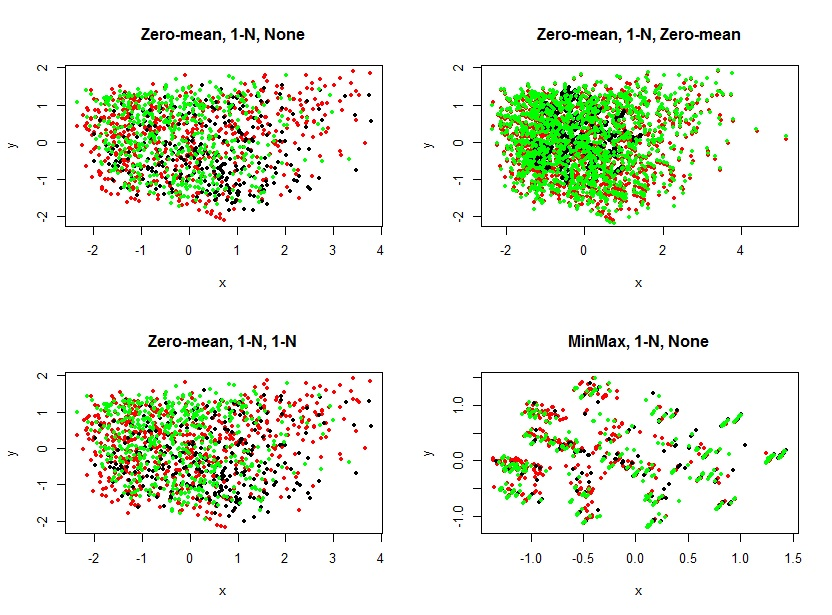
\includegraphics[scale=\figurescaling]{figures/db1/dim_reduction.jpg}
\caption{Dimensional Reduction applied on different preprocessing techniques (Numerical, Categorical, Binary)
\label{fig:db1-dimred}}
\end{figure}


\subsection{Logistic Regression}
We applied different values of the parameter $C$ (Inverse of regularization strength) and tried the algorithm in both polynomial and linear ways. Whole the process was also done using two preprocessing methods mentioned before.

The F1-score of the result is shown in Table\ref{table:db1-logisticregression}. As it's shown in Table\ref{table:db1-logisticregression}, changing the parameter $C$ doesn't cause any significant difference in results while $0.1$ seems to be slightly better. Also while $PreProc1$ seems better in result in some records, $PreProc2$ seems to be more stable and indifference against changing the highest exponent.


\begin{table}[p]
\begin{center}
\begin{tabular}{|c|c|c|c|c|}
\hline \multicolumn{2}{ |c| }{C} & 0.1 & 2 & 5 \\

\hline \multicolumn{1}{ |c| }{\multirow{6}{*}{Highest exponent} } & 1 & \minibox{0.50\\ 0.51} & \minibox{0.49 \\ 0.50} & \minibox{0.49 \\ 0.50} \\

\cline{2-5} & 5 & \minibox{0.55 \\ 0.53} & \minibox{0.55 \\ 0.52} & \minibox{0.56 \\ 0.53} \\

\cline{2-5} & 10 & \minibox{\textbf{0.56} \\ 0.50} & \minibox{0.54 \\ 0.51} & \minibox{0.54 \\ 0.52} \\

\cline{2-5} & 21 & \minibox{0.39 \\ 0.52} & \minibox{0.39 \\ 0.52} & \minibox{0.39 \\ 0.52} \\

\cline{2-5} & 33 & \minibox{0.34 \\ 0.52} & \minibox{0.34 \\ 0.52} & \minibox{0.34 \\ 0.53} \\

\cline{2-5} & 44 & \minibox{0.24 \\ 0.52} & \minibox{0.24 \\ 0.52} & \minibox{0.24 \\ 0.53} \\

\hline
\end{tabular}

\caption{Contraceptive Method Choice - Logistic Regressions F1-score ($PreProc1$, $PreProc2$)}
\label{table:db1-logisticregression}
\end{center}
\end{table}

We applied the best result ($C=0.1$, $Highest exponent=10$) on test dataset and the result is shown in Table\ref{table:db1-logisticregression-test}. The result is slightly worse than the best result of Cross Validation dataset.


\begin{table}[p]
\begin{center}
\begin{tabular}{|c|c|c|c|c|}
\hline Class & Precision & Recall & F1-score & Support \\

\hline 0 & 0.59 & 0.62 & 0.60 & 126\\
\hline 1 & 0.54 & 0.22 & 0.32 & 67\\
\hline 2 & 0.46 & 0.61 & 0.53 & 102\\
\hline avg / total & 0.53 & 0.53 & 0.51 & 295\\
\hline
\end{tabular}

\caption{Contraceptive Method Choice - Logistic Regressions on Test dataset}
\label{table:db1-logisticregression-test}
\end{center}
\end{table}

\subsection{Decision Tree}
We applied two criteria for decision tree: $gini$ and $entropy$. As before, we repeated it for two preprocessing methods mentioned before.

The F1-score of the result is shown in Table\ref{table:db1-decisiontree}. $Gini$ seems to be a better criterion measure for the algorithm. Also in this case, $PreProc1$ seems better than $PreProc2$.


\begin{table}[p]
\begin{center}
\begin{tabular}{|c|c|}
\hline Criterion & F-Score \\

\hline Gini & \minibox{\textbf{0.48}\\ 0.47} \\

\hline Entropy & \minibox{0.46\\ 0.43} \\

\hline
\end{tabular}

\caption{Contraceptive Method Choice - Decision Tree F1-score ($PreProc1$, $PreProc2$)}
\label{table:db1-decisiontree}
\end{center}
\end{table}

We applied again the best result ($Criterion=Gini$) on test dataset and the result is shown in Table\ref{table:db1-decisiontree-test}. The result is again slightly worse than the best result of Cross Validation dataset.


\begin{table}[p]
\begin{center}
\begin{tabular}{|c|c|c|c|c|}
\hline Class & Precision & Recall & F1-score & Support \\

\hline 0 & 0.55 & 0.57 & 0.56 & 126\\
\hline 1 & 0.33 & 0.34 & 0.34 & 67\\
\hline 2 & 0.42 & 0.39 & 0.41 & 102\\
\hline avg / total & 0.46 & 0.46 & 0.46 & 295\\
\hline
\end{tabular}

\caption{Contraceptive Method Choice - Decision Tree on Test dataset}
\label{table:db1-decisiontree-test}
\end{center}
\end{table}

\subsection{$k$-nearest neighbor}
Since the data is so blended, we run the algorithm many times with different values of Number of Neighbors parameter. As before, the process is repeated two times for preprocessing methods.

The F1-score of the result is shown in Table\ref{table:db1-knn}. Running the algorithm with $30$ neighbors as parameter seems to be the best result. Also in this case, $PreProc1$ seems better than $PreProc2$.


\begin{table}[p]
\begin{center}
\begin{tabular}{|c|c|}
\hline Number of Neighbors & F-Score \\

\hline 1 & \minibox{0.42\\ 0.45} \\
\hline 5 & \minibox{0.47\\ 0.46} \\
\hline 10 & \minibox{0.51\\ 0.43} \\
\hline 20 & \minibox{0.51\\ 0.45} \\
\hline 30 & \minibox{\textbf{0.56}\\ 0.47} \\
\hline 40 & \minibox{0.54\\ 0.49} \\
\hline 50 & \minibox{0.54\\ 0.47} \\

\hline
\end{tabular}

\caption{Contraceptive Method Choice - K Nearest Neighbors  F1-score ($PreProc1$, $PreProc2$)}
\label{table:db1-knn}
\end{center}
\end{table}

We applied again the best result ($Number of Neighbors=30$) on test dataset and the result is shown in Table\ref{table:db1-knn-test}. The result is again slightly worse than the best result of Cross Validation dataset.


\begin{table}[p]
\begin{center}
\begin{tabular}{|c|c|c|c|c|}
\hline Class & Precision & Recall & F1-score & Support \\

\hline 0 & 0.61 & 0.60 & 0.60 & 126\\
\hline 1 & 0.48 & 0.43 & 0.45 & 67\\
\hline 2 & 0.49 & 0.54 & 0.51 & 102\\
\hline avg / total & 0.54 & 0.54 & 0.54 & 295\\
\hline
\end{tabular}

\caption{Contraceptive Method Choice - K Nearest Neighbors on Test dataset}
\label{table:db1-knn-test}
\end{center}
\end{table}

\subsection{Support Vector Machine}
Kernel and value $C$ (Inverse of regularization strength) are two factors considered in running SVM algorithm. Different kernels like RBF (Radial Basis Function), Linear, Polynomial and Sigmoid are applied on the dataset.

Since the result of Sigmoid are significantly bad, in Table\ref{table:db1-svm} we only show the results of RBF, Linear and Polynomial. Again $PreProc1$ seems better in result rather than $PreProc2$. As it's expected, RBF have the best results among other kernels.


\begin{table}[p]
\begin{center}
\begin{tabular}{|c|c|c|c|c|c|c|}
\hline \multicolumn{2}{ |c| }{C} & 1 & 5 & 10 & 20 & 50 \\

\hline \multicolumn{1}{ |c| }{\multirow{2}{*}{Kernel} } & Linear & \minibox{0.48\\ 0.49} & \minibox{0.49 \\ 0.50} & \minibox{0.49 \\ 0.49} & \minibox{0.49 \\ 0.48} & \minibox{0.49 \\ 0.49} \\

\cline{2-7} & RBF & \minibox{\textbf{0.57} \\ 0.47} & \minibox{0.56 \\ 0.52} & \minibox{0.55 \\ 0.53} & \minibox{0.53 \\ 0.51}  & \minibox{0.52 \\ 0.51} \\

\cline{2-7} & Polynomial & \minibox{0.27 \\ 0.26} & \minibox{0.51 \\ 0.35} & \minibox{0.53 \\ 0.45} & \minibox{0.54 \\ 0.47}  & \minibox{0.53 \\ 0.48} \\

\hline
\end{tabular}

\caption{Contraceptive Method Choice - SVM F1-score ($PreProc1$, $PreProc2$)}
\label{table:db1-svm}
\end{center}
\end{table}

We applied the best result ($C=1$, $Kernel=RBF$) on test dataset and the result is shown in Table\ref{table:db1-svm-test}. The result is slightly worse than the best result of Cross Validation dataset.


\begin{table}[p]
\begin{center}
\begin{tabular}{|c|c|c|c|c|}
\hline Class & Precision & Recall & F1-score & Support \\

\hline 0 & 0.60 & 0.65 & 0.63 & 126\\
\hline 1 & 0.54 & 0.33 & 0.41 & 67\\
\hline 2 & 0.50 & 0.58 & 0.54 & 102\\
\hline avg / total & 0.55 & 0.55 & 0.55 & 295\\
\hline
\end{tabular}

\caption{Contraceptive Method Choice - SVM on Test dataset}
\label{table:db1-svm-test}
\end{center}
\end{table}


\subsection{Neural Networks}
Number of hidden layers as well as number of nodes in each hidden layer are two important factors in result of neural network algorithm. 

Usually the number of nodes in hidden layer should be at least twice as number of nodes in input layer (number of attributes). The results are shown in Table\ref{table:db1-nn}. Again $PreProc1$ seems better in result rather than $PreProc2$. As it's expected, RBF have the best results among other kernels.


\begin{table}[p]
\begin{center}
\begin{tabular}{|c|c|c|c|c|c|c|}
\hline \multicolumn{2}{ |c| }{Number of Nodes} & 30 & 60 & 90 & 120 & 150 \\

\hline \multicolumn{1}{ |c| }{\multirow{2}{*}{Number of Hidden Layers} } & 1 & \minibox{0.34\\ 0.28} & \minibox{0.27 \\ 0.32} & \minibox{0.35 \\ 0.32} & \minibox{\textbf{0.37} \\ 0.34} & \minibox{0.26 \\ 0.35} \\

\cline{2-7} & 2 & \minibox{0.18 \\ 0.18} & \minibox{0.26 \\ 0.18} & \minibox{0.26 \\ 0.26} & \minibox{0.26 \\ 0.18}  & \minibox{0.26 \\ 0.08} \\

\hline
\end{tabular}

\caption{Contraceptive Method Choice - Neural Network F1-score ($PreProc1$, $PreProc2$)}
\label{table:db1-nn}
\end{center}
\end{table}

We applied the best result ($Number of Layers=1$, $Number of Nodes=120$) on test dataset. The result is shown in Table\ref{table:db1-nn-test}. The result is as good as the best result of Cross Validation dataset.


\begin{table}[p]
\begin{center}
\begin{tabular}{|c|c|c|c|c|}
\hline Class & Precision & Recall & F1-score & Support \\

\hline 0 & 0.53 & 0.26 & 0.35 & 126\\
\hline 1 & 0.26 & 0.42 & 0.32 & 67\\
\hline 2 & 0.37 & 0.46 & 0.41 & 102\\
\hline avg / total & 0.42 & 0.37 & 0.37 & 295\\
\hline
\end{tabular}
\caption{Contraceptive Method Choice - Neural Network on Test dataset}
\label{table:db1-nn-test}
\end{center}
\end{table}


\subsection{Comparison}
Table\ref{table:db1-comparison} compares the between best run of each algorithm on Test dataset based on the value of precision, recall, F1-score, learning time and prediction time.

\begin{table}[p]
\begin{center}
\begin{tabular}{|p{5cm}|c|c|c|p{2cm}|p{2cm}|}
\hline Algorithm & Precision & Recall & F1-score & Training Time & Prediction Time \\
\hline Logistic Regression, PreProc1, C=0.1, Exponent=10 & 0.53 & 0.53 & 0.51 & 01.528 & 00.323\\
\hline Decision Tree, PreProc1, Criterion=Gini & 0.46 & 0.46 & 0.46 & \textbf{00.019} & \textbf{00.049}\\
\hline K Nearest Neighbors, PreProc1, NN=30 & 0.54 & 0.54 & 0.54 & 00.029 & 00.662 \\
\hline SVM, PreProc1, Kernel=RBF, C=1 & \textbf{0.55} & \textbf{0.55} & \textbf{0.55} & 00.281 & 00.189\\
\hline Neural Network, PreProc1, NL=1, NN=120 & 0.42 & 0.37 & 0.37 & 03.202 & 00.251\\
\hline
\end{tabular}
\caption{Contraceptive Method Choice - Comparison}
\label{table:db1-comparison}
\end{center}
\end{table}

Since SVM tends to have a better results among the other algorithm, its confusion matrix is depicted in Table \ref{table:db1-confusionmatrix}

\begin{table}[p]
\begin{center}
\begin{tabular}{|c|c|c|c|}
\hline \backslashbox{Class}{Predicted} & 1 & 2 & 3  \\
\hline 1 & \textbf{80} & 9 & 37\\
\hline 2 & 16 & \textbf{28} & 23\\
\hline 3 & 30 & 11 & \textbf{60}\\
\hline
\end{tabular}
\caption{Contraceptive Method Choice - Confusion Matrix}
\label{table:db1-confusionmatrix}
\end{center}
\end{table}

Based on achieved results, following points can be infered:
\begin{itemize}
\item Using Standard Deviation instead of MinMax leads to better results in all cases.
\item SVM has the best result and the result is rather consistent in different runs.
\item Surprisingly, KNN has a really good results such that it's completely comparable with SVM. Since it's a lazy learner algorithm, in the case of need it can be replaced with SVM.
\item Neural Network has a very bad result. Usually precision is better than recall and smaller collections are worse in results.
\item Analyzing confusion matrix and the results of runs show us that class $1$ and $3$ are mistaken more often. As it is mentioned before class $1$ and $3$ stand for No-use and Short-term.
\item While training and prediction time are usually less than one minute and not time consuming, NN algorithm tends to have about three times longer training time than the others.
\item Decision Tree is the fastest algorithm among the others
\item While KNN is expected to have a more prediction time than training, the same situation can be seen for Decision Tree. The reason is probably because of short amount of data and time which makes the situation not appropriate for judgment.
\end{itemize}
